\documentclass[format=sigconf, nonacm=true, review=true, screen=true]{acmart}

\usepackage[utf8]{inputenc}
\usepackage{xcolor}
\usepackage{fancyvrb}
\usepackage{minted}
\usepackage{xspace}
\usepackage{hyperref}
\usepackage{subfigure}

% Use this instead of caption to remove acmart description warnings
\newcommand{\mycaption}[1]{\Description{#1}\caption{#1}}
\newcommand{\TODO}[1]{\textcolor{red}{TODO: #1}}

% For highlighting some texts
% \newcommand{\red}[1]{\textcolor{red}{#1}}

% This appears to fix some font problem...
\DeclareRobustCommand{\ttfamily}{\fontencoding{T1}\fontfamily{lmtt}\selectfont}

% Junk for acmart:
\setcopyright{acmcopyright}
\copyrightyear{2022}
\acmYear{2022}
\acmDOI{N/A}
\acmBooktitle{N/A}

\title{Speech Onset Detection using sEEG}
\author{Jennie Chen}
\author{Kevin Jin}
\author{Eric Conlon}
\authorsaddresses{}
\date{2022-12-17}

\begin{document}

\begin{abstract}

In this project, we construct models of speech onset learned from sEEG signals. We compare conventional ML against deep learning on the task and in both cases perform binary classification with better performance than random chance. There were many challenges in working with the sEEG dataset we used, and we wonder if the benefits of high signal-to-noise ratio outweigh the problems of generalizability.

\end{abstract}

\maketitle

\section{Introduction}

Speech-related brain-computer interfaces (BCIs) can provide new communication strategies for people with speaking disabilities. One popular research topic in this area is direct speech reconstruction, but it is difficult to approach this due to the high dimensionality of the input data and of the intermediate representations as well as the difficulty with reconstructing intelligible speech waveforms. \cite{saha2019deep} A simpler problem is to predict the onset of intended speech. This could be used for voice-handicapped persons to be able to indicate their intent to communicate. For instance, one practical use would be to control/toggle on a light bulb when a patient is trying to indicate their needs to a caretaker.

Different brain signal monitoring modalities have been used in BCI, such as surface electroencephalography (EEG), electrocorticography (ECoG), etc. \cite{herff2020potential}. In comparison, ECoG has a much higher spatial and temporal resolution than EEG \cite{parvizi2018promises}. Since ECoG is measured directly on the cortex, it is able to measure high gamma band activity which is involved in speech production \cite{herff2020potential}. In recent years stereotactic electroencephalography (sEEG) signals have emerged in BCI studies. In contrast to ECoG, which uses a highly localized grid of electrodes, sEEG is capable of measuring the potential in a number of brain regions. The acquisition of sEEG signals requires penetrating depth electrodes that can obtain data from even deeper brain structures than ECoG \cite{herff2020potential}. This allows for the possibility to investigate the role of different brain structures in speech production. As for its data quality, sEEG has a signal-to-noise ratio of up to 100 times higher than surface EEG, which makes it a very attractive signal source. On the clinical front, it is also slightly less invasive and has fewer surgical complications than ECoG grid implantation \cite{herff2020potential}.

Overall, sEEG's high signal-to-noise ratio and the potential it offers in investigating deeper and diverse regions makes it an interesting modality to investigate. Specifically, we are interested in its application in speaker-independent speech onset detection.

% Comment from TA: your motivation can be made stronger. You mentioned that the "sentence spotting" task has already been done nicely with EEG signals, so what is the motivation to improve it further with sEEG

\section{Related Work}

Researchers have been successful in synthesizing speech through ECoG signals measured in the ventral sensorimotor cortex as activity in this brain region is related to articulatory movements \cite{chartier2018encoding, anumanchipalli2018intelligible}.

\TODO{talk about the 2 papers from the presentation + seizure detection paper. find some more papers in speech production, onset/event detection, network structures, etc.}

% “The type of ML algorithm was categorized into four groups: Standard supervised ML includes popular algorithms such as support vector machines (SVM), K-nearest neighbors (KNN), single-layered artificial neural networks (ANN), linear discriminant analysis (LDA) and any others that did not fit the definition of deep learning. Deep learning algorithms include recurrent neural networks (RNN), convolutional neural networks (CNN) and multi-layered neural networks” [Decoding Intracranial EEG With Machine Learning: A Systematic Review]

% LSTMs are stable and powerful in modelling long-term dependencies [https://proceedings.neurips.cc/paper/2015/file/07563a3fe3bbe7e3ba84431ad9d055af-Paper.pdf]

% Seizure detection using LSTMs \cite{xu2020seizure}

\section{Methods}

\subsection{Data}

It is extremely difficult to collect sEEG signals, since it requires surgical implantation of electrodes in a patient's brain (which, of course, is beyond the scope of this project). As such we rely on a publicly-available dataset of spoken word prompts with simultaneous audio and sEEG recordings. \cite{verwoert2022dataset} This dataset represents experimental results from 10 patients speaking 100 words (from a corpus of Dutch words) as prompted. Between words, patients focused on a fixation cross. The location of intracranial electrodes varies between patients, but they are labeled with anatomical location. There are a total of 1103 recorded electrode signals with between 54 and 127 per patient. This dataset is relatively small, so it is challenging to apply learning techniques that require many examples to converge. However, there is reason to believe that the signal content of the dataset is good: the researchers who assembled the dataset were able to reconstruct an audio spectrogram in log-mel space with a linear transformation of the sEEG spectrogram.

\subsection{Clustering channels}

We find that predicting speech onsets with single-channel observations is unreliable, so we focus our efforts on multi-channel observations. However, we must overcome a significant disadvantage of intracranial EEG: the variability of probe placements between participants. Contrast this to surface EEG, in which the spatial arrangement of channels is fixed by the particular hardware used. This dataset contains spatial coordinates and rough functional areas for each channel collected from each participant, but it is not clear how to group these channels for analysis. Some functional areas are over- or underrepresented across participants, and the total number of channels varies. It might be possible to incorporate all channels' data in a single observation for certain types of models with hidden states, but we prefer to try a principled and consistent method for grouping channels. With a chosen a number of \textit{clusters} (32) we use Bisecting K-Means to derive spatial positions for these clusters from the set of positions of all channels across all participants. Then for each participant and each cluster we assign the channel from that participant that is closest to the cluster centroid (and has not been previously assigned). With these assignments we are able to work with an ordered list of channels for each participant where channels in corresponding positions have some spatial similarity. We also include spatial position in our features to allow models to compensate for the approximate nature of our assignments.

\TODO{show graph of cluster locations + maybe list of channels assigned to each}


\subsection{Task}

Our primary task is to predict speech onset from sEEG signals. Previous work has successfully performed this ``sentence spotting'' (SS) task with a high level of accuracy and precision on EEG datasets. \cite{sakthi2021keyword} We follow their model: intervals from 500ms before and 250ms after sentence onset are labeled 1 and other intervals 0. With this dataset, there are approximately 110,000 unique positive examples, but of course there are many correlations, as they are drawn from a limited pool of speakers and words. In practice there are far fewer positive examples, as multi-channel classification is virtually required.

\subsection{Signal processing}

The dataset contains sEEG signals sampled at 1024 Hz. These sampling rates are more than adequate (brain waves are generally quoted in the range of 1-100 Hz and above). In their reconstruction experiment \cite{verwoert2022dataset}, researchers post-processed their sEEG signals by bandpass-filtering between 70-170 Hz and bandstop-filtering around 50 Hz. Though SS with deep learning \cite{sakthi2021keyword} can directly operate on the time domain signal, we calculate some frequency domain features for use with baseline learning methods. These features include band power for four common frequency ranges used in EEG analysis: theta (4-7 Hz), alpha (8-12 Hz), beta (13-25 Hz), and gamma (30-45 Hz).

\subsection{Data preparation}

While the dataset has markers for stimuli, it does not have any for speech onset. We create markers in the form of timestamps for each of the onsets. Initially, we attempted to use librosa's onset detection function directly on each of the speech signals, but realized that the audio is littered with noise caused by patient movement. We also tried applying a bandpass filter for the natural frequency range of human voice, but this did not seem to help with the onset detection. Our final solution was to first leverage the structure of the audio data, which is that each word is shown to the patient for 2 seconds, followed by 1 second of fixation, so we assume that the onset can only occur after the word is shown and that it will end before the fixation period. We iterate over every stimulus window, apply Viterbi decoding to separate silence and non-silence regions, and then apply librosa's onset detection function. Each of these onsets is saved as a marker in .aiff format. There are however a few instances where our assumptions do not hold. For example, a few words are pronounced during the fixation period. In these edge cases, we save a list of the words that could not be detected and manually mark the onsets in audio editing software.

With speech onset marks, we derive start and end points for positive windows of 750ms. For negative examples, we randomly choose onsets at least 500ms away from any speech onset. With this scheme we ensure a balance of positive and negative examples as well as complete channel data for every window. These examples are augmented with cluster assigments and frequency-domain features, and they are saved for quick access in model training and testing.

We run our experiments on several prepared datasets: One is a randomly selected 80:10:10 train/validation/test split across all participants and all times. (We realize that we are biasing our model by learning hidden temporal variables, but we found it necessary to use as many samples as possible for training.) The rest are 1-participant holdout sets used to test generalizability.

\subsection{Evaluation metrics}
To evaluate the performance of our models, we primarily plotted receiver operating characteristic (ROC) curves and compared the area under the curve (AUC) for the test dataset, giving us a standardized metric to compare the performance between different models. The ROC curve is a common method to assess the performance of binary classifiers, where the true positive rate is plotted on the y-axis and the false positive rate is plotted on the x-axis for various classification thresholds. The AUC value summarizes the performance of a model for all classification thresholds. 

After initial screening based on AUC values, we also use other metrics to assess model performance. These metrics include the accuracy ($A$), precision ($P$), recall ($R$), and F1-score ($F1$), which are defined as follows:
\[P=\frac{TP}{TP+FP} \;\; R=\frac{TP}{TP+FN}\]
\[A=\frac{TP+TN}{TP+TN+FP+FN} \;\; F1=\frac{2PR}{P+R}\]
where $TP$ is the number of true positives, $TN$ is the number of true negatives, $FP$ is the number of false positives, and $FN$ is the number of false negatives. Precision tells us the proportion of true speech onsets out of all predicted speech onsets and recall tells us the proportion of speech onsets out of all actual speech onsets. The F1-score balances precision and recall into one evaluation metric.

\subsection{Learning models}

\subsubsection{Classical machine learning models as baseline}
As a baseline, we tried various traditional machine learning models with single channel classification using the power band features extracted from the sEEG signals (where the class is predicted from the features of a single channel). These models, which included a Support Vector Classifier, Gaussian Naive Bayes, and a Random Forest model generally did not perform well. We then tried multi-channel classification with our clustered data, which resulted in improved performances. We settled for a Random Forest Classifier which operates on band power features as our baseline model, as this was the model that showed the best performance.

\subsubsection{GRU and LSTM model}
We turned to literature to find deep learning models to apply to our data. We first tried the sentence spotter gated-recurrent unit (GRU) model developed by Sakthi et al \cite{sakthi2021keyword}. to perform binary classification task using multi-channel raw EEG data. In their paper, the GRU model was shown to have the best performance in detecting speech onsets, compared to the other model architectures (Long Short-Term Memory (LSTM) and Naive Bayes) that the authors explored. \cite{sakthi2021keyword} The GRU model consisted of 2 GRU layers (with 512 and 256 units), and a fully-connected layer, with a sigmoid activation function to perform the prediction \cite{sakthi2021keyword}. We followed the same architecture in our GRU model. We also tried a LSTM model, with a similar architecture, replacing the GRU units with LSTM units. The GRU and LSTM model architectures are shown in Fig. \ref{fig:gru-arch} and \ref{fig:lstm-arch}, respectively.

\begin{figure}[H]
    \centering
    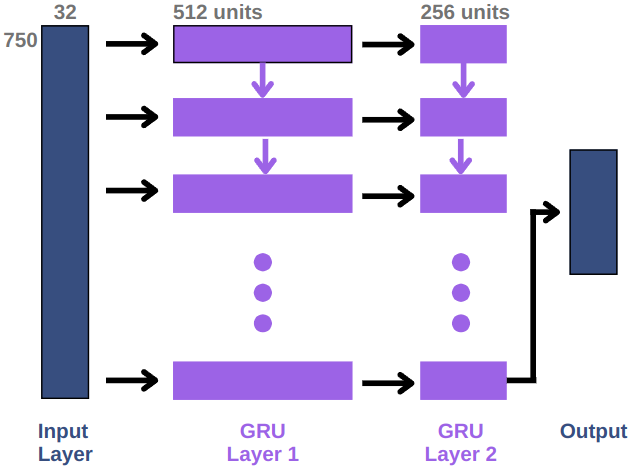
\includegraphics[width=\columnwidth]{figures/gru-arch.png}
    \caption{The GRU model architecture.}
    \label{fig:gru-arch}
\end{figure}

\begin{figure}[H]
    \centering
    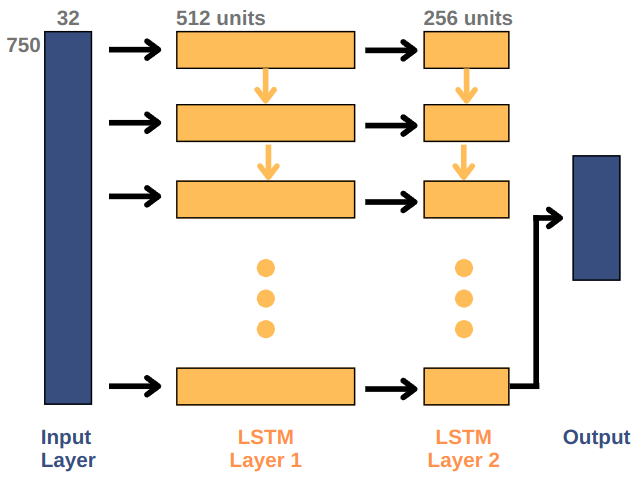
\includegraphics[width=\columnwidth]{figures/lstm-arch.png}
    \caption{The LSTM model architecture.}
    \label{fig:lstm-arch}
\end{figure}

\subsubsection{Combined CNN and LSTM models}
In this approach, we use one 1D convolution layer combined with two LSTM layers to extract both spatial and temporal information, as well as two fully-connected layers. This approach uses a similar model architecture to seizure detection methods \cite{xu2020seizure}
We experimented with both ways of arranging the CNN and LSTM sections and determined that CNN-LSTM yields better performance. The architectures of the two models are shown in Fig. \ref{fig:lstm-cnn-arch} and \ref{fig:cnn-lstm-arch}. Since CNN-LSTM yields the best performance out of all of the models we tried, Section \ref{sec:modeltraining} will mostly detail its tuning process as well as present an analysis of the effects of some of the hyperparameters.

\begin{figure}[H]
    \centering
    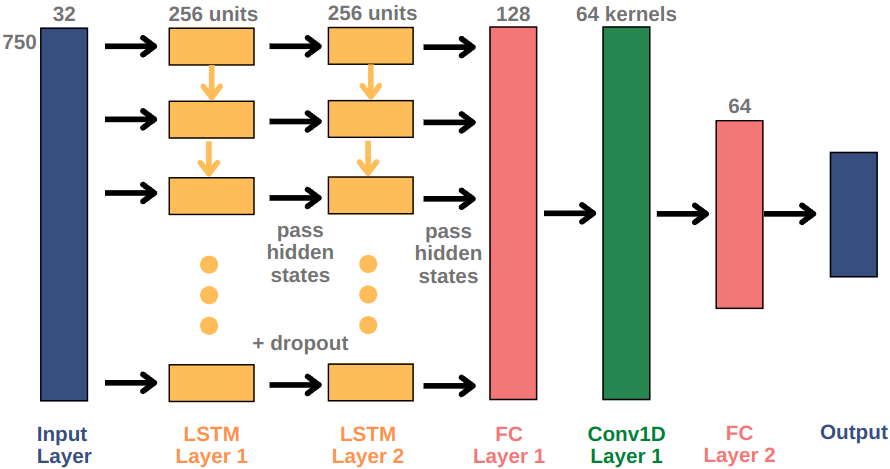
\includegraphics[width=\columnwidth]{figures/lstm-cnn-arch.png}
    \caption{The LSTM-CNN model architecture.}
    \label{fig:lstm-cnn-arch}
\end{figure}

\begin{figure}[H]
    \centering
    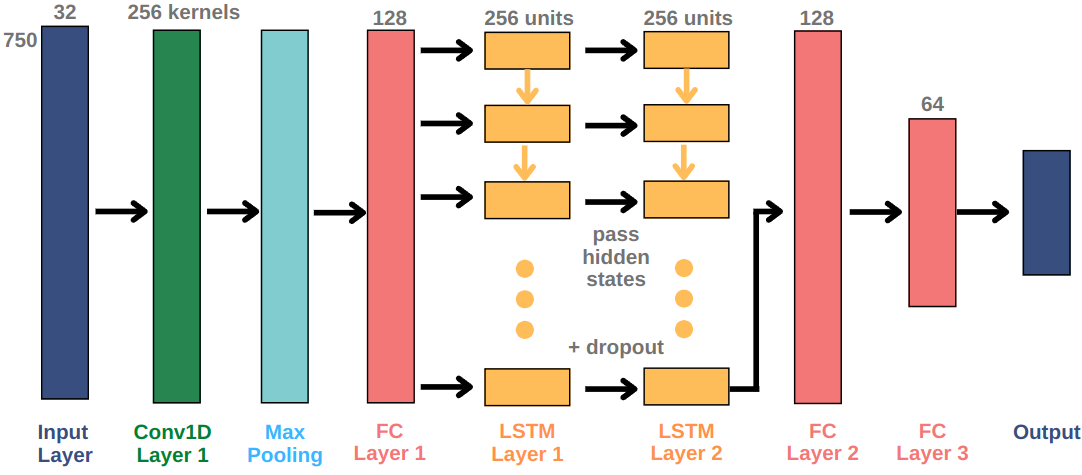
\includegraphics[width=\columnwidth]{figures/cnn-lstm-arch.png}
    \caption{The CNN-LSTM model architecture.}
    \label{fig:cnn-lstm-arch}
\end{figure}

\subsubsection{LSTM-Feature model}
So far, we've trained traditional ML models on features extracted from the dataset (namely, power in various frequency bands) as well as end-to-end deep learning models on EEG data only. We attempt to combine both input data sources in a hybrid approach in our LSTM-Feature model, using our extracted features together with the raw EEG data to perform classification as shown in Figure \ref{fig:lstm_feature_model}. The model takes EEG data as input, passes it through LSTM model, while also taking features as input, passing them through a fully-connected layer. These neurons are then concatenated and used together as input through a MLP to identify whether a given window contains a speech onset. This model was originally trained on the dataset without any jitter added, but we later switched to the jitter dataset, as jitter seemed to slightly improve the model's learning capablities.

\begin{figure}[H]
    \centering
    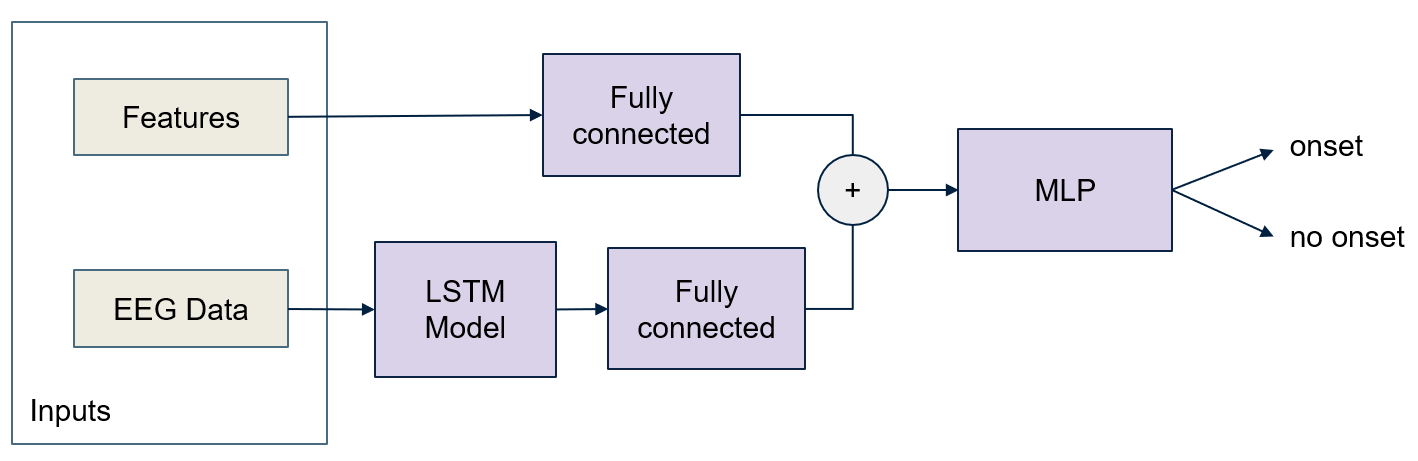
\includegraphics[width=\columnwidth]{figures/lstm-feature-model.png}
    \caption{The LSTM-feature model architecture.}
    \label{fig:lstm_feature_model}
\end{figure}

\subsubsection{GRU-Feature model}
Seeing our success with the LSTM-feature model, we then tried a GRU-feature model, which utilizes the same idea. This model had the same architecture as in Figure \ref{fig:lstm_feature_model}, but with the LSTM module replaced with a GRU. This model was also trained on the dataset with jitter.

\subsection{Model tuning and analysis} \label{sec:modeltraining}
At the start of the training process, we first wanted to verify the performance of the various deep learning approaches on a high level, so we fixed a few hyperparameters such as the number of epochs (30), the batch size (64), the optimization algorithm (Adam with default Keras parameters) \cite{adamoptimizer, chollet2015keras}, and the EEG sample generation method (no jitter). With these fixed hyperparameters, we determined that the CNN-LSTM method had the best initial performance by comparing the score given by the area under the ROC curve. Then, we hand-tuned the hyperparameters of the more promising models to try to improve their performance.

During the training and preliminary tuning process of the CNN-LSTM model, we encountered many issues. The first issue common to all of the deep learning models was the problem of overfitting to the dataset, as is evidenced by the high training scores and lower testing scores. This is likely due to the size of our dataset being too small to represent all possible input values. To mitigate this, we experimented with adding jitter to the data samples in order to increase the total number of samples to be generated. Specifically for the CNN-LSTM model, we also used regularization methods such as adding a L2 regularization term (explicit regularization), as well as dropout layers and early stopping (implicit regularization) \cite{srivastava14a}.

During this process, we also encountered the exploding gradient problem. Sometimes during the training process, the loss would suddenly explode to NaN values. When we encountered this, we first experimented with adding L2 regularization, decreasing the learning rate, and lowering the dropout amount, but this did not seem to solve the issue.
We also used weight initialization methods such as Glorot and He initializations in Keras \cite{Glorot2010UnderstandingTD, HeZR015}.
Finally, we added gradient clipping as detailed in \cite{pascanu2012} and this was highly effective at mitigating the exploding gradient issue.

% https://stackoverflow.com/questions/69427103/gradient-exploding-problem-in-a-graph-neural-network
% https://stackoverflow.com/questions/37232782/nan-loss-when-training-regression-network

Once the exploding gradient problem was resolved, we moved onto tuning the hyperparameters and architecture of the CNN-LSTM model in a grid search over a total of 29 trials. We experimented with the addition of a fully-connected layer between the CNN and LSTM sections, the number of training epochs, the dropout rate, the training batch size, the number of CNN layers, kernels and kernel size, the size of the MaxPool layer, the number of units in the LSTM layers, and the amount of jitter. After each set of trials we hand-picked the best hyperparameter based on its performance metrics. Sometimes, if the performance is too similar, the tie-breaker is chosen by the option that would yield in the shorter training time. The ROC curves and confusion matrices for all of the trials are shown in Appendix \ref{app:CNN-LSTM_Grid} and a summary of the results can be seen in Fig. \ref{fig:cnn-lstm_grid_table}.

To highlight some of the more interesting results, the number of training epochs (trials 3, 4, 5, 1 and 6), as expected, had an effect on the performance of the model as shown in Fig. \ref{fig:cnn-lstm_training_epochs}. As the model trains for longer epochs, the AUC increases until the training process reaches 20 epochs, then it begins to decrease. As mentioned previously, the model tends to overfit due to the size of the dataset, so performing early stopping would make sense in this case.

\begin{figure}
    \centering
    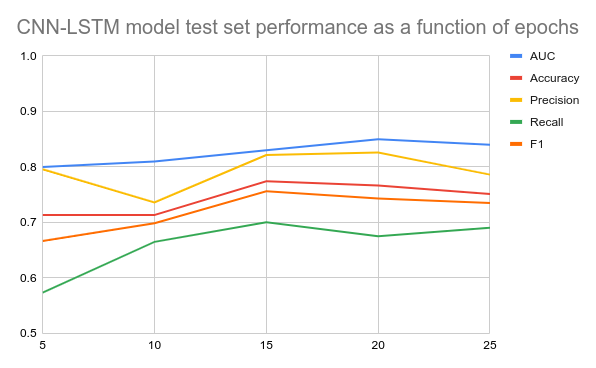
\includegraphics[width=\columnwidth]{figures/cnn-lstm_test_epochs.png}
    \caption{Performance parameters of the CNN-LSTM model as a function of the number of training epochs}
    \label{fig:cnn-lstm_training_epochs}
\end{figure}

Another hyperparameter that had a significant effect on the performance was the batch size (trials 9, 7 and 10), with 128 as a suitable middle ground. This makes sense since large batch sizes do not generalize well \cite{KeskarMNST16}. Also, with the smaller batch size, although the gradients no longer explode to NaN, we still sometimes observe that the loss at the end of certain epochs would have very large numbers, which indicates that it is unstable.

Surprisingly, the CNN section architecture did not seem to affect the performance as much (Number of Conv1D layers: trials 11, 12 and 7; Number of kernels: 11, 13, 14, 15 and 16; Kernel size: trials 17, 14, 18 and 19). However, as we can see by the performances of the regular LSTM and CNN-LSTM, the presence of the convolution layer definitely made a difference.
On the other hand, for the LSTM section architecture, increasing the number of LSTM units in each of the layers seemed to have a positive effect on the performance.

We also tested the maxpooling size of the pooling layer after the convolutional layer (trials 24, 23, 22, 14, 21 and 20). One interesting observation is that without the pooling layer, the exploding gradient issue came back. As for the other trials, it seemed that there is also a tradeoff between large and small maxpooling sizes, as the middle value yielded the best results.

Through visual analysis of the confusion matrices, we can see that the CNN-LSTM models perform better at recognizing true negatives than true positives, with the exception of trials 12 and 28. Interestingly, trial 28 was the only trial whose data input did not have any jitter. We can speculate that when the onset is at a fixed time delay, the model has an easier time recognizing the onset pattern. However, when we add jitter, it becomes harder to recognize the onset pattern, but since the model sees more negative examples, it is better at recognizing when a non-valid pattern.

\section{Results}
Table \ref{tab:result-summary} summarizes the final performance of our various models.
% we can report other metrics too like accuracy, f1 score, precision, recall, etc. maybe training AUC too?
\begin{table}[H]
  \caption{Summary of evaluation results}
  \label{tab:result-summary}
  \begin{tabular}{cc}
    \toprule
    Model & Test AUC\\
    \midrule
    Random Forest & 0.67\\
    LSTM & 0.68\\
    GRU & 0.72\\
    LSTM-CNN & 0.79\\
    CNN-LSTM & 0.89\\
    LSTM-Feature & 0.78\\
    GRU-Feature & 0.81\\
  \bottomrule
\end{tabular}
\end{table}

\subsection{Hybrid approach}
Our results suggest that a hybrid approach, utilizing both the raw EEG data and the extracted power band features can improve the learning capabilities of deep models. Specifically, the LSTM-Feature and GRU-Feature models both outperformed the LSTM and GRU models respectively (which operated on the raw EEG data alone) by a signficant margin. The hybrid approach also outperformed the baseline Random Forest Classifier, which operated only on the extracted power band features. Hence, it appears that combining the information from raw EEG data and expert domain knowledge in the form of power band features results in better performance than either method alone.

\subsection{Feature visualization}
We visualized our single-channel power band features by plotting the mean and standard deviations across for the positive and negative windows in each frequency range, to gain a better understanding of our dataset (Figure \ref{fig:barplot_mean_std_visualization}). A delta band (1-3 Hz) was later added to our power band features as well. Generally, the difference between the mean powers of positive and negative windows did not appear to be very distinguishable, with the mean powers being much less than the standard deviation for a particular frequency range. Furthermore, the positive windows had a higher mean, but this effect diminished for higher frequencies (e.g. beta, gamma). The highest powers were observed in the lower frequency bands (e.g. delta, theta, alpha), and the power diminished for higher frequency bands (e.g. beta, gamma). Interestingly, the positive windows also had a much higher standard deviation in power values than the negative windows.

\begin{figure}[H]
     \centering
     \begin{subfigure}
         \centering
         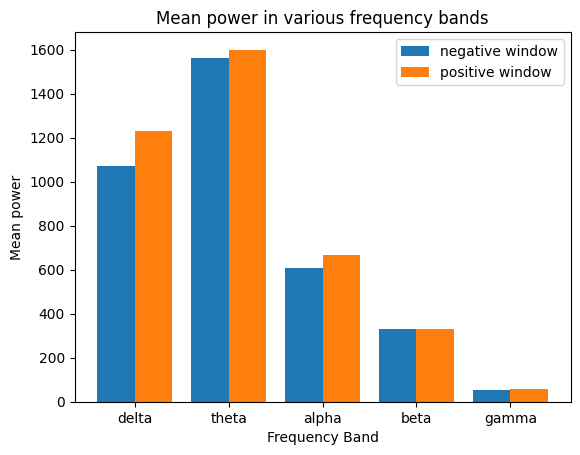
\includegraphics[width=0.48\columnwidth]{figures/bar-power-all-mean.png}
     \end{subfigure}
     \begin{subfigure}
         \centering
         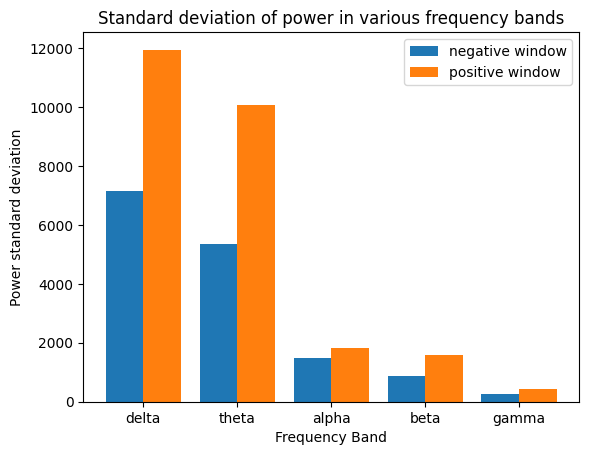
\includegraphics[width=0.48\columnwidth]{figures/bar-power-all-stdev.png}
     \end{subfigure}
     \caption{Plots of the mean and standard deviation in various frequency bands across all channels.}
     \label{fig:barplot_mean_std_visualization}
\end{figure}

\subsection{Cluster visualization}
To better understand our clustering algorithm, we plotted the difference in mean power for each cluster in the various frequency bands using a 3D scatter plot in Figure \ref{fig:cluster_visualization}. For each cluster point (x, y, z), which corresponds to the mean position of the cluster, the difference between the mean  power in positive windows and mean power in negative windows is plotted in terms of intensity using a colorbar. The colorbar was scaled by the minimum and maximum power differences for a particular frequency range. We observe that the clustering algorithm generates clusters that are fairly scattered to cover the 3D region, with a few clusters in close proximity. From this plot, we can identify regions in the brain that pertain to speech production (i.e. regions with larger differences - the extremes of the color scale). It seems that the regions with the largest differences varies based on the frequency range being examined (e.g. the gamma band emphasizes different clusters compared to the theta band). However, it's worth noting that these computed differences tended to be quite small compared to the magnitude of the power values. Hence, we did not use these differences to inform our models, but it may be an interesting area to explore more in the future.

% It would be nice if we could label them (a), (b), etc. but idk how to do that in latex haha
\begin{figure}[H]
     \centering
     \begin{subfigure}
         \centering
         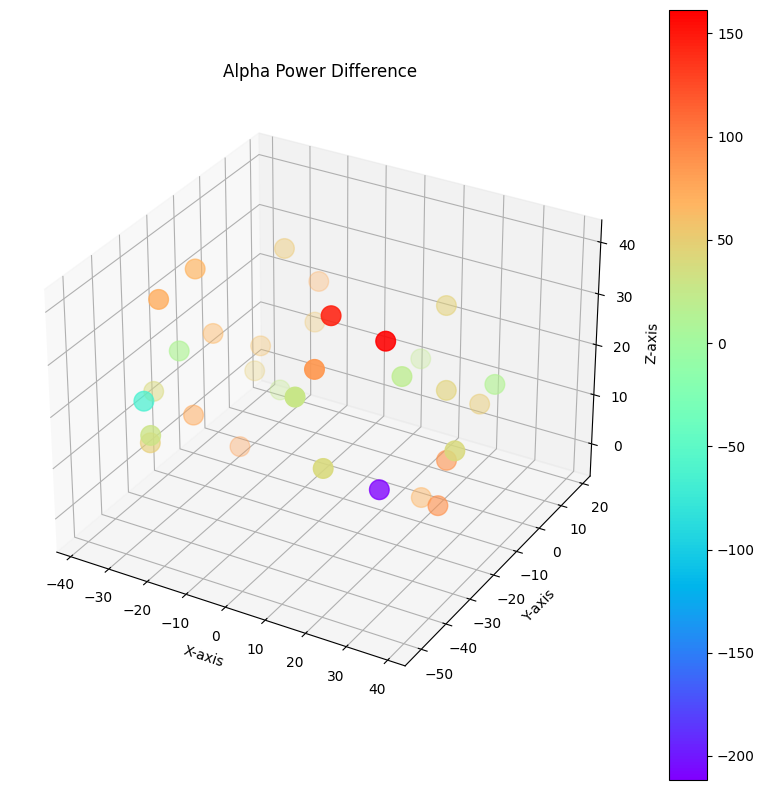
\includegraphics[width=0.48\columnwidth]{figures/cluster-alpha.png}
     \end{subfigure}
     \begin{subfigure}
         \centering
         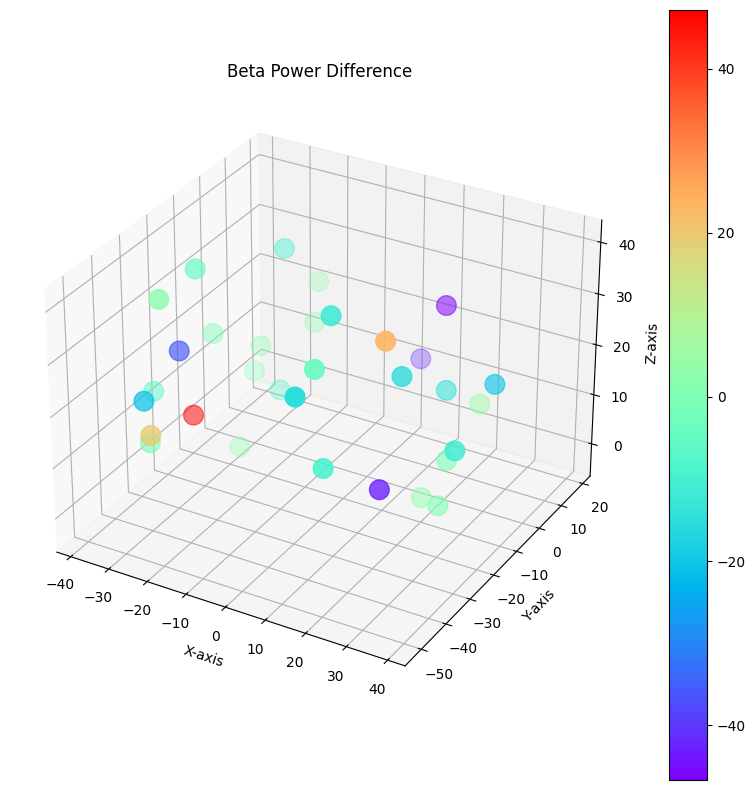
\includegraphics[width=0.48\columnwidth]{figures/cluster-beta.png}
     \end{subfigure}
     \begin{subfigure}
         \centering
         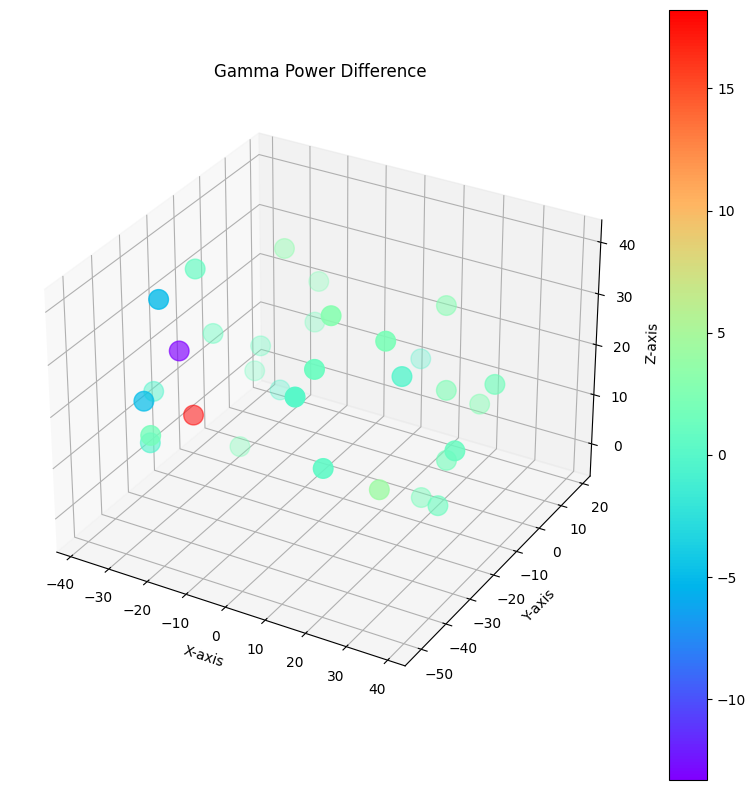
\includegraphics[width=0.48\columnwidth]{figures/cluster-gamma.png}
     \end{subfigure}
     \begin{subfigure}
         \centering
         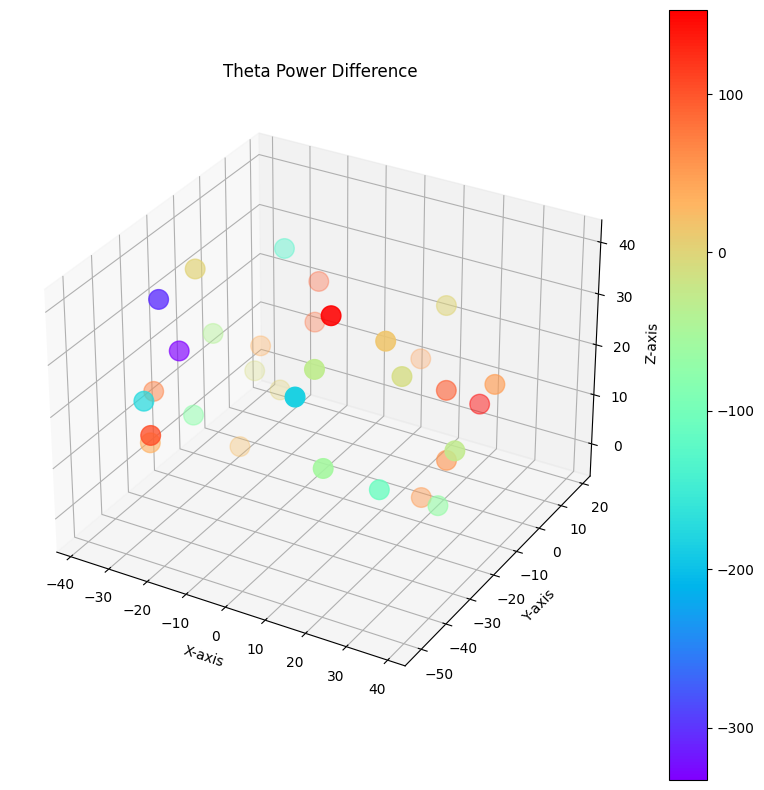
\includegraphics[width=0.48\columnwidth]{figures/cluster-theta.png}
     \end{subfigure}
    \caption{Plots of theta, alpha, beta, and gamma power in our 32 clusters.}
    \label{fig:cluster_visualization}
\end{figure}

\TODO{Live results}

Etc...

\section{Conclusion}
% EEG data contains information that can be used to detect speech onsets
% While the various models we’ve developed to identify onsets work better than random chance, there is still quite some room for improvement
% This may be due to an inherent limitation of the information contained within EEG data or difficulty distinguishing meaningful features from all the noise that is typically present in EEG signals
% There may also be variations across participants 

Despite the addition of jitter to increase the sample size and the use of various regularization methods, overfitting remains an issue in our various models. This is a limitation of our dataset.

% Other evaluation metrics to assess performance
% Combining DL with traditional ML (eg. SVM-LSTM)
% Try with single channel, more sophisticated channel clustering methods, etc.
% Choosing specific channels (areas in brain related to imagined speech or speech production)
% Using more expert domain knowledge to perform heavier featurization 
% Evaluate across different participants

% Talk about choosing specific channels https://www.frontiersin.org/articles/10.3389/fnins.2021.642251/full

\newpage
\bibliographystyle{ACM-Reference-Format}
\bibliography{biosignals-report}

\newpage
\onecolumn
\appendix
\section{ROC Curves and Confusion Matrices} \label{App:ROC_Curves}
The ROC curves and confusion matrices for our various models are presented here.

\renewcommand{\thefigure}{A.\arabic{figure}}
\setcounter{figure}{0}

\begin{figure}[H]
     \centering
     \begin{subfigure}
         \centering
         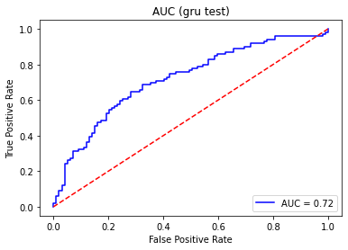
\includegraphics[width=0.24\columnwidth]{figures/gru-roc.png}
     \end{subfigure}
     \begin{subfigure}
         \centering
         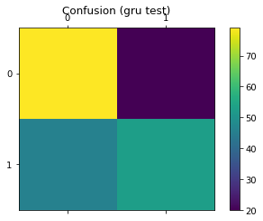
\includegraphics[width=0.24\columnwidth]{figures/gru-cm.png}
     \end{subfigure}
     \caption{GRU model}
     \label{fig:gru-roc-cm}
     
     \centering
     \begin{subfigure}
         \centering
         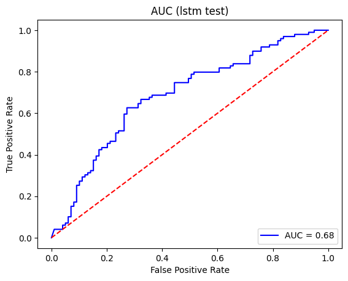
\includegraphics[width=0.24\columnwidth]{figures/lstm-roc.png}
     \end{subfigure}
     \begin{subfigure}
         \centering
         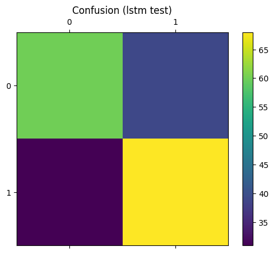
\includegraphics[width=0.24\columnwidth]{figures/lstm-cm.png}
     \end{subfigure}
     \caption{LSTM model}
     \label{fig:lstm-roc-cm}

     \centering
     \begin{subfigure}
         \centering
         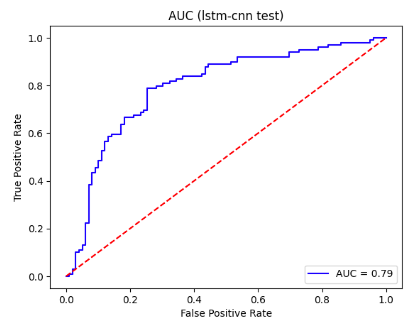
\includegraphics[width=0.24\columnwidth]{figures/lstm-cnn-roc.png}
     \end{subfigure}
     \begin{subfigure}
         \centering
         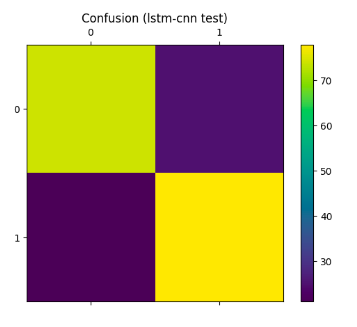
\includegraphics[width=0.24\columnwidth]{figures/lstm-cnn-cm.png}
     \end{subfigure}
     \caption{LSTM-CNN model}
     \label{fig:lstm-cnn-roc-cm}

     \centering
     \begin{subfigure}
         \centering
         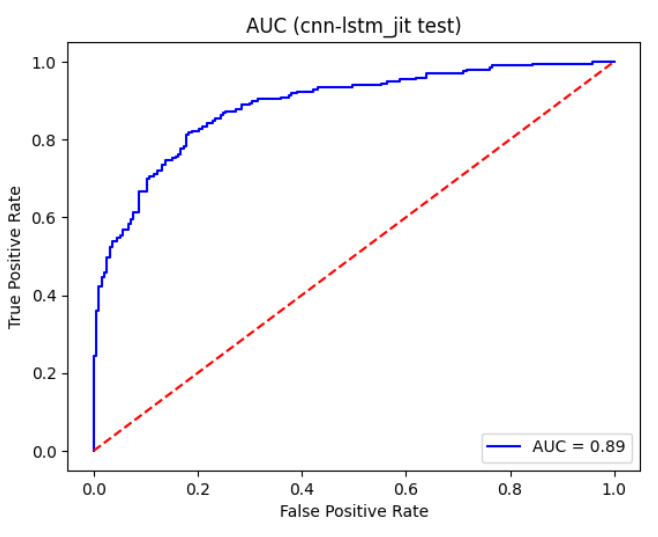
\includegraphics[width=0.24\columnwidth]{figures/cnn-lstm-roc.png}
     \end{subfigure}
     \begin{subfigure}
         \centering
         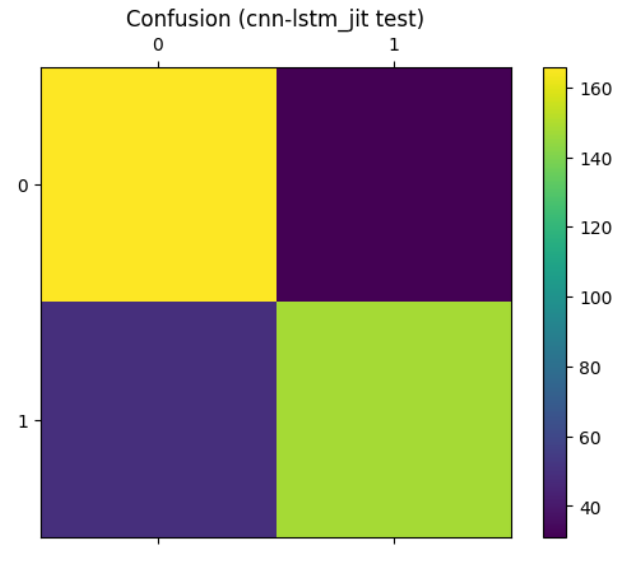
\includegraphics[width=0.24\columnwidth]{figures/cnn-lstm-cm.png}
     \end{subfigure}
     \caption{CNN-LSTM model}
     \label{fig:cnn-lstm-roc-cm}
 \end{figure}

\newpage
\begin{figure}[H]
     \centering
     \begin{subfigure}
         \centering
         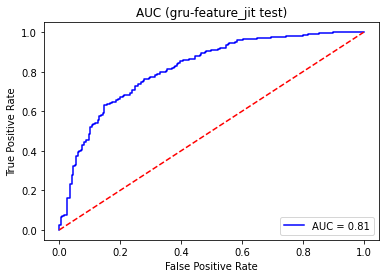
\includegraphics[width=0.24\columnwidth]{figures/gru-feature-roc.png}
     \end{subfigure}
     \begin{subfigure}
         \centering
         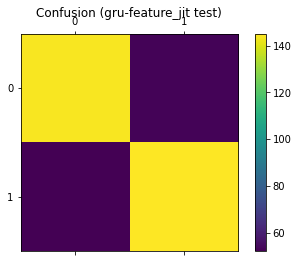
\includegraphics[width=0.24\columnwidth]{figures/gru-feature-cm.png}
     \end{subfigure}
     \caption{GRU-Feature model}
     \label{fig:gru-feature-roc-cm}
     
     \centering
     \begin{subfigure}
         \centering
         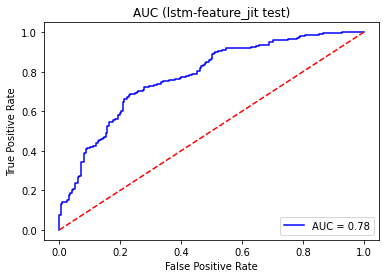
\includegraphics[width=0.24\columnwidth]{figures/lstm-feature-roc.png}
     \end{subfigure}
     \begin{subfigure}
         \centering
         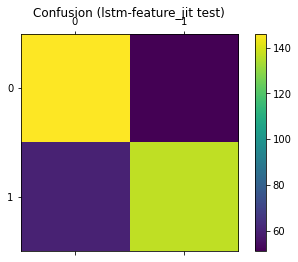
\includegraphics[width=0.24\columnwidth]{figures/lstm-feature-cm.png}
     \end{subfigure}
     \caption{LSTM-Feature model}
     \label{fig:lstm-feature-roc-cm}
\end{figure}

\newpage
\section{CNN-LSTM Grid Search} \label{app:CNN-LSTM_Grid}
\renewcommand{\thefigure}{B.\arabic{figure}}
\setcounter{figure}{0}
\begin{figure}[H]
    \centering
    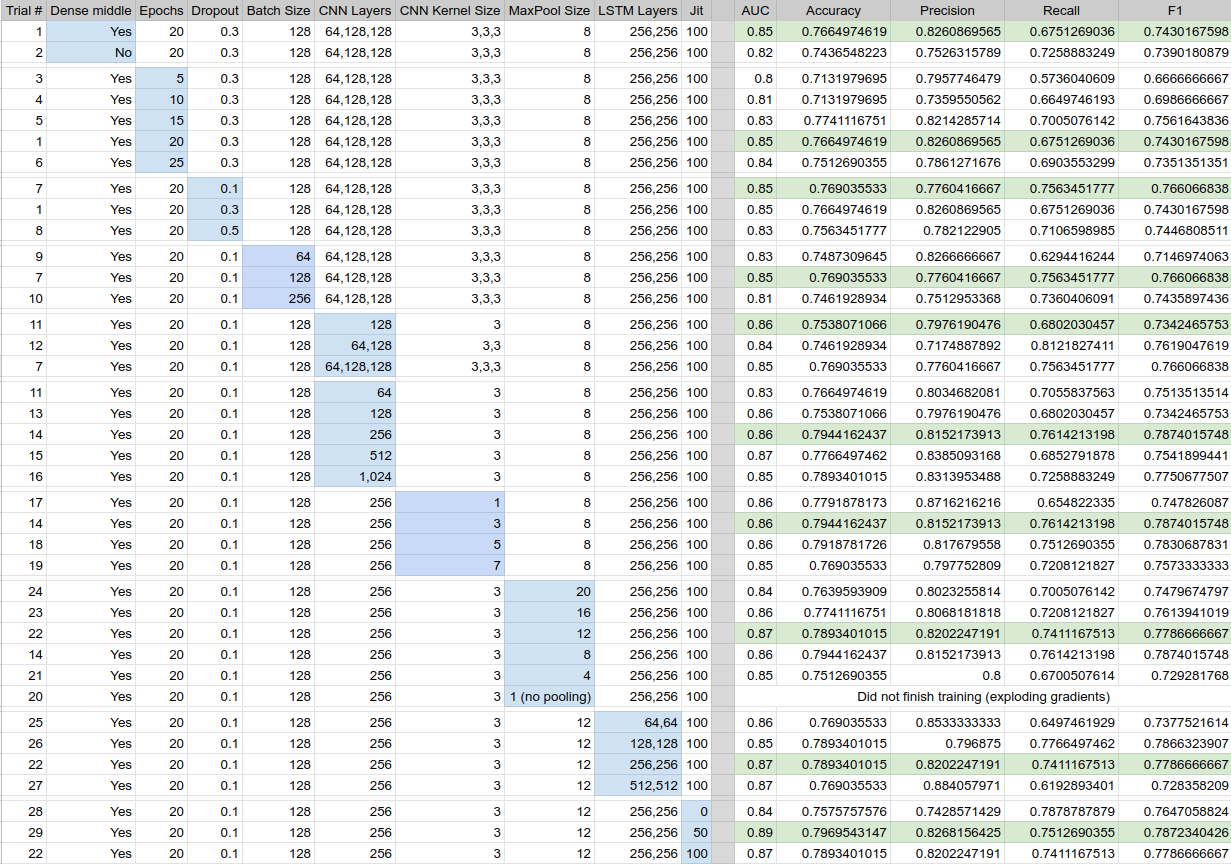
\includegraphics[width=\columnwidth]{figures/cnn-lstm_grid_search.png}
    \caption{Summary of results from the hyperparameter grid search}
    \label{fig:cnn-lstm_grid_table}
\end{figure}

\begin{figure}
    \centering
    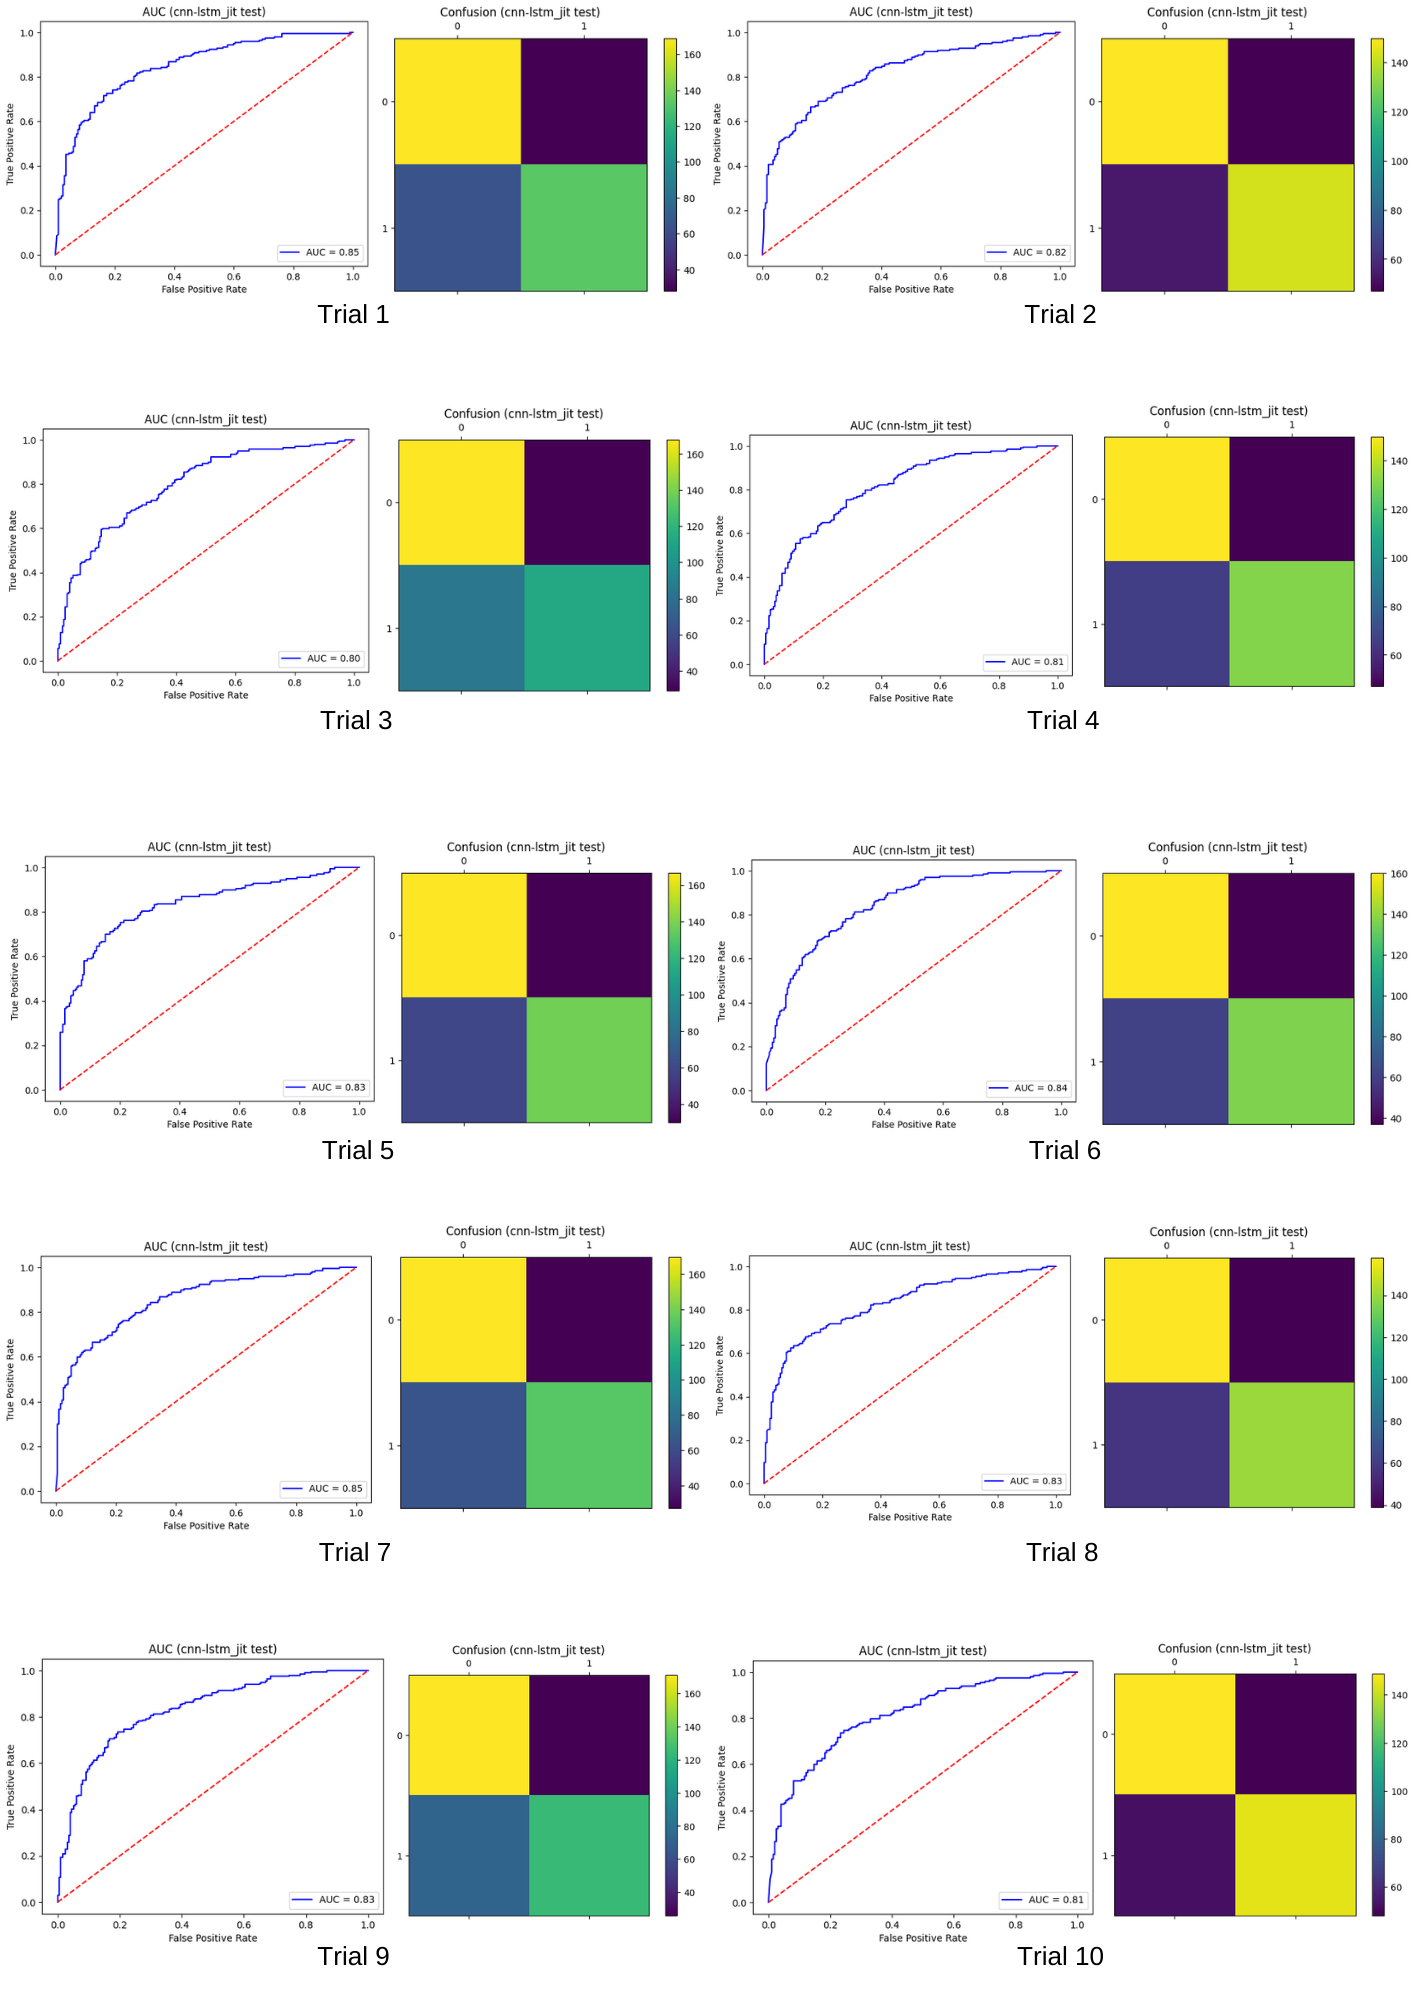
\includegraphics[width=0.9\columnwidth]{figures/cnn-lstm_1.png}
    \label{fig:cnn-lstm_1}
\end{figure}
\begin{figure}
    \centering
    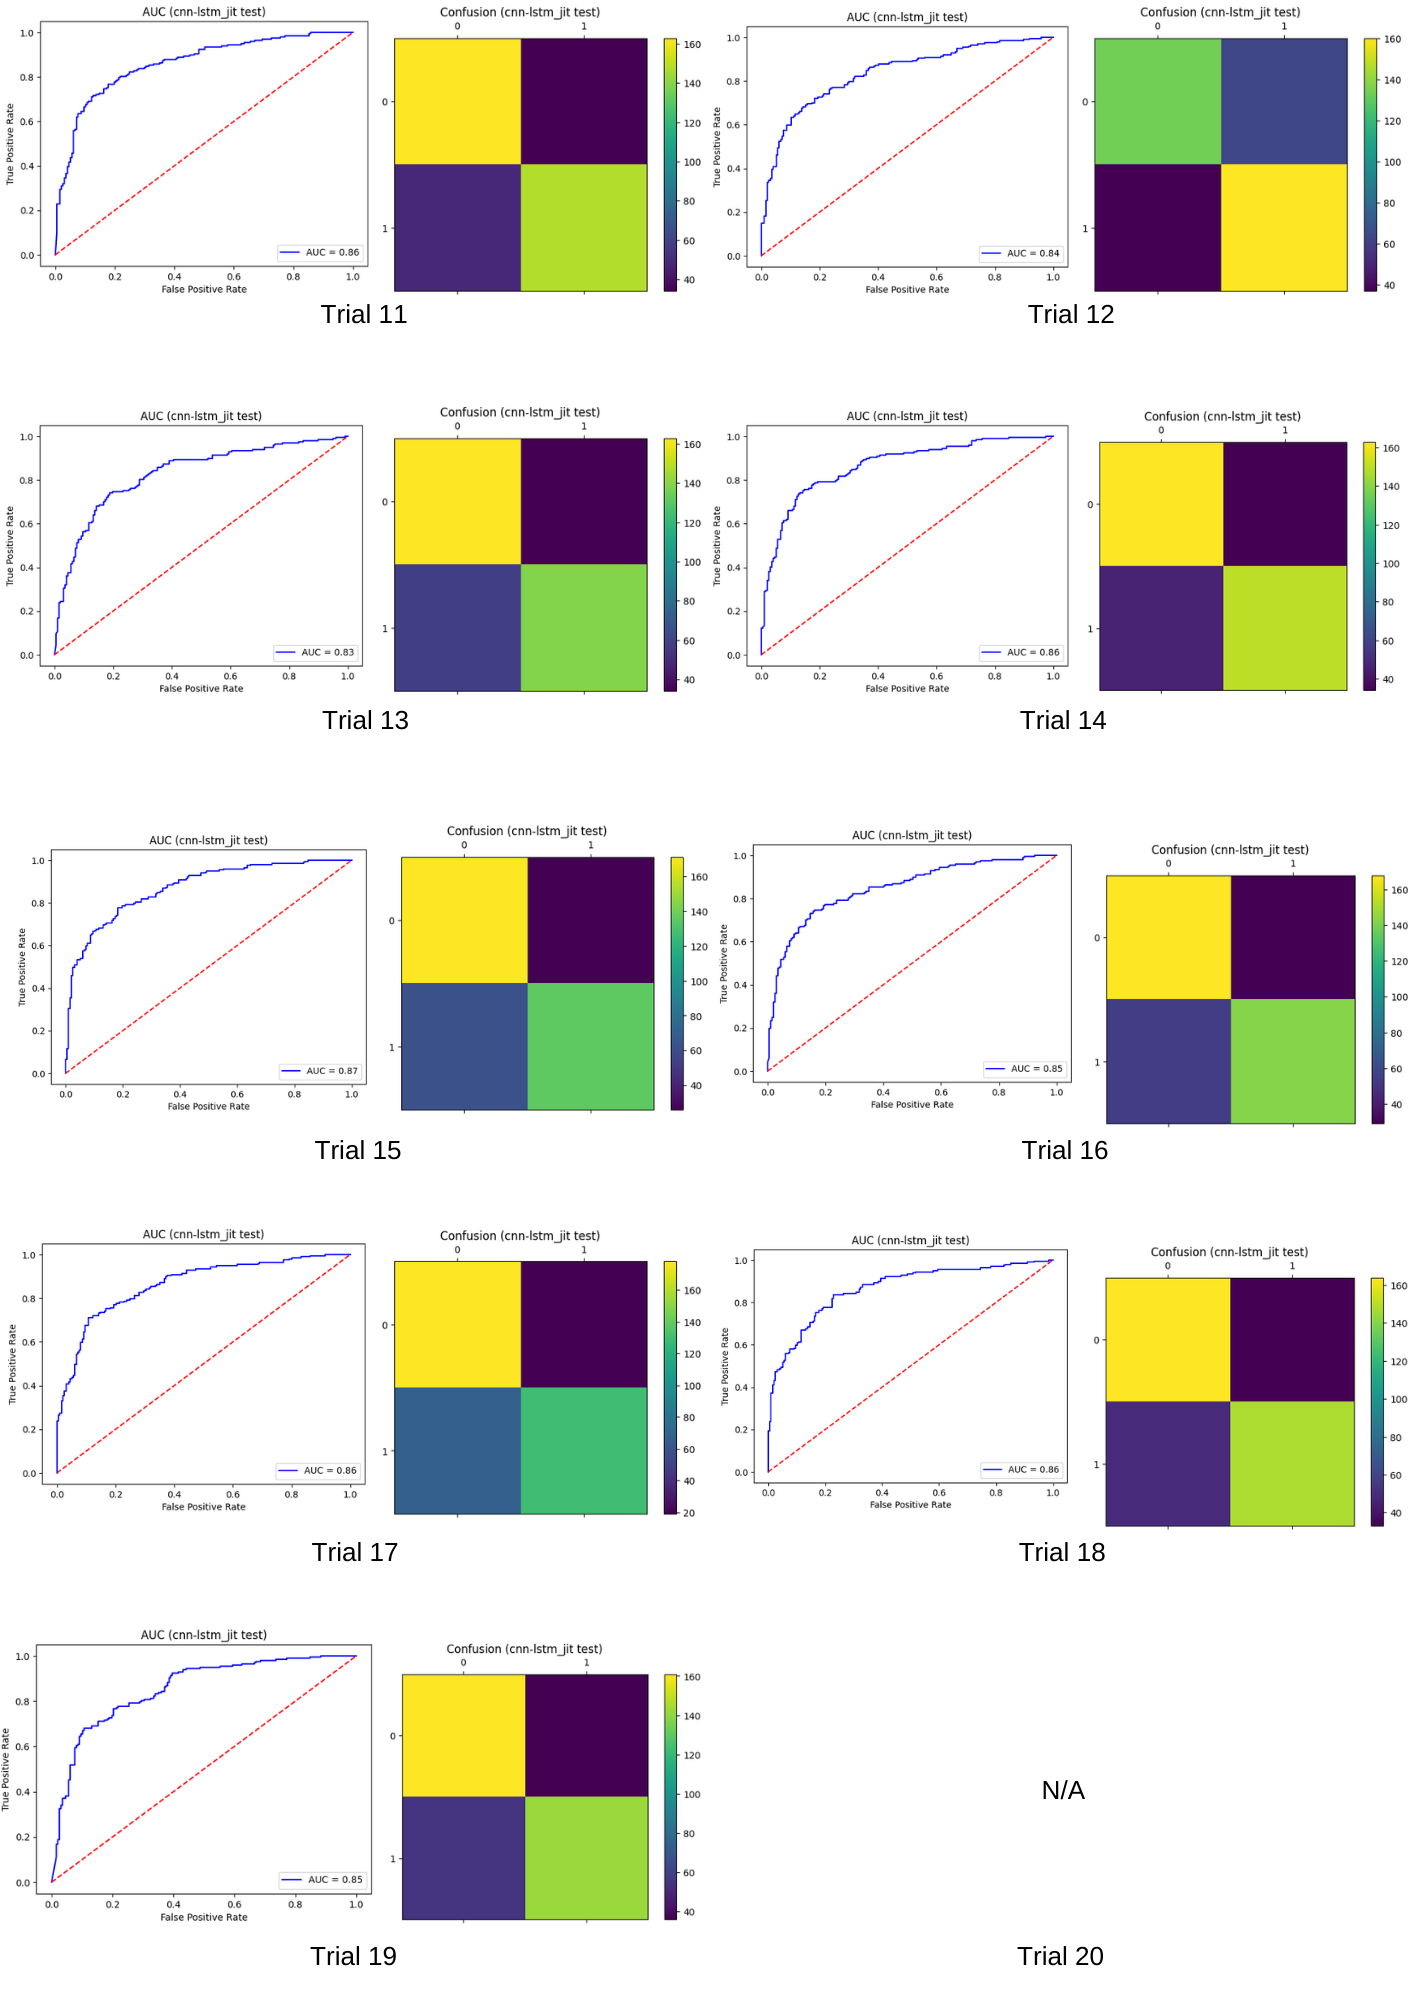
\includegraphics[width=0.9\columnwidth]{figures/cnn-lstm_2.png}
    \label{fig:cnn-lstm_2}
\end{figure}
\begin{figure}
    \centering
    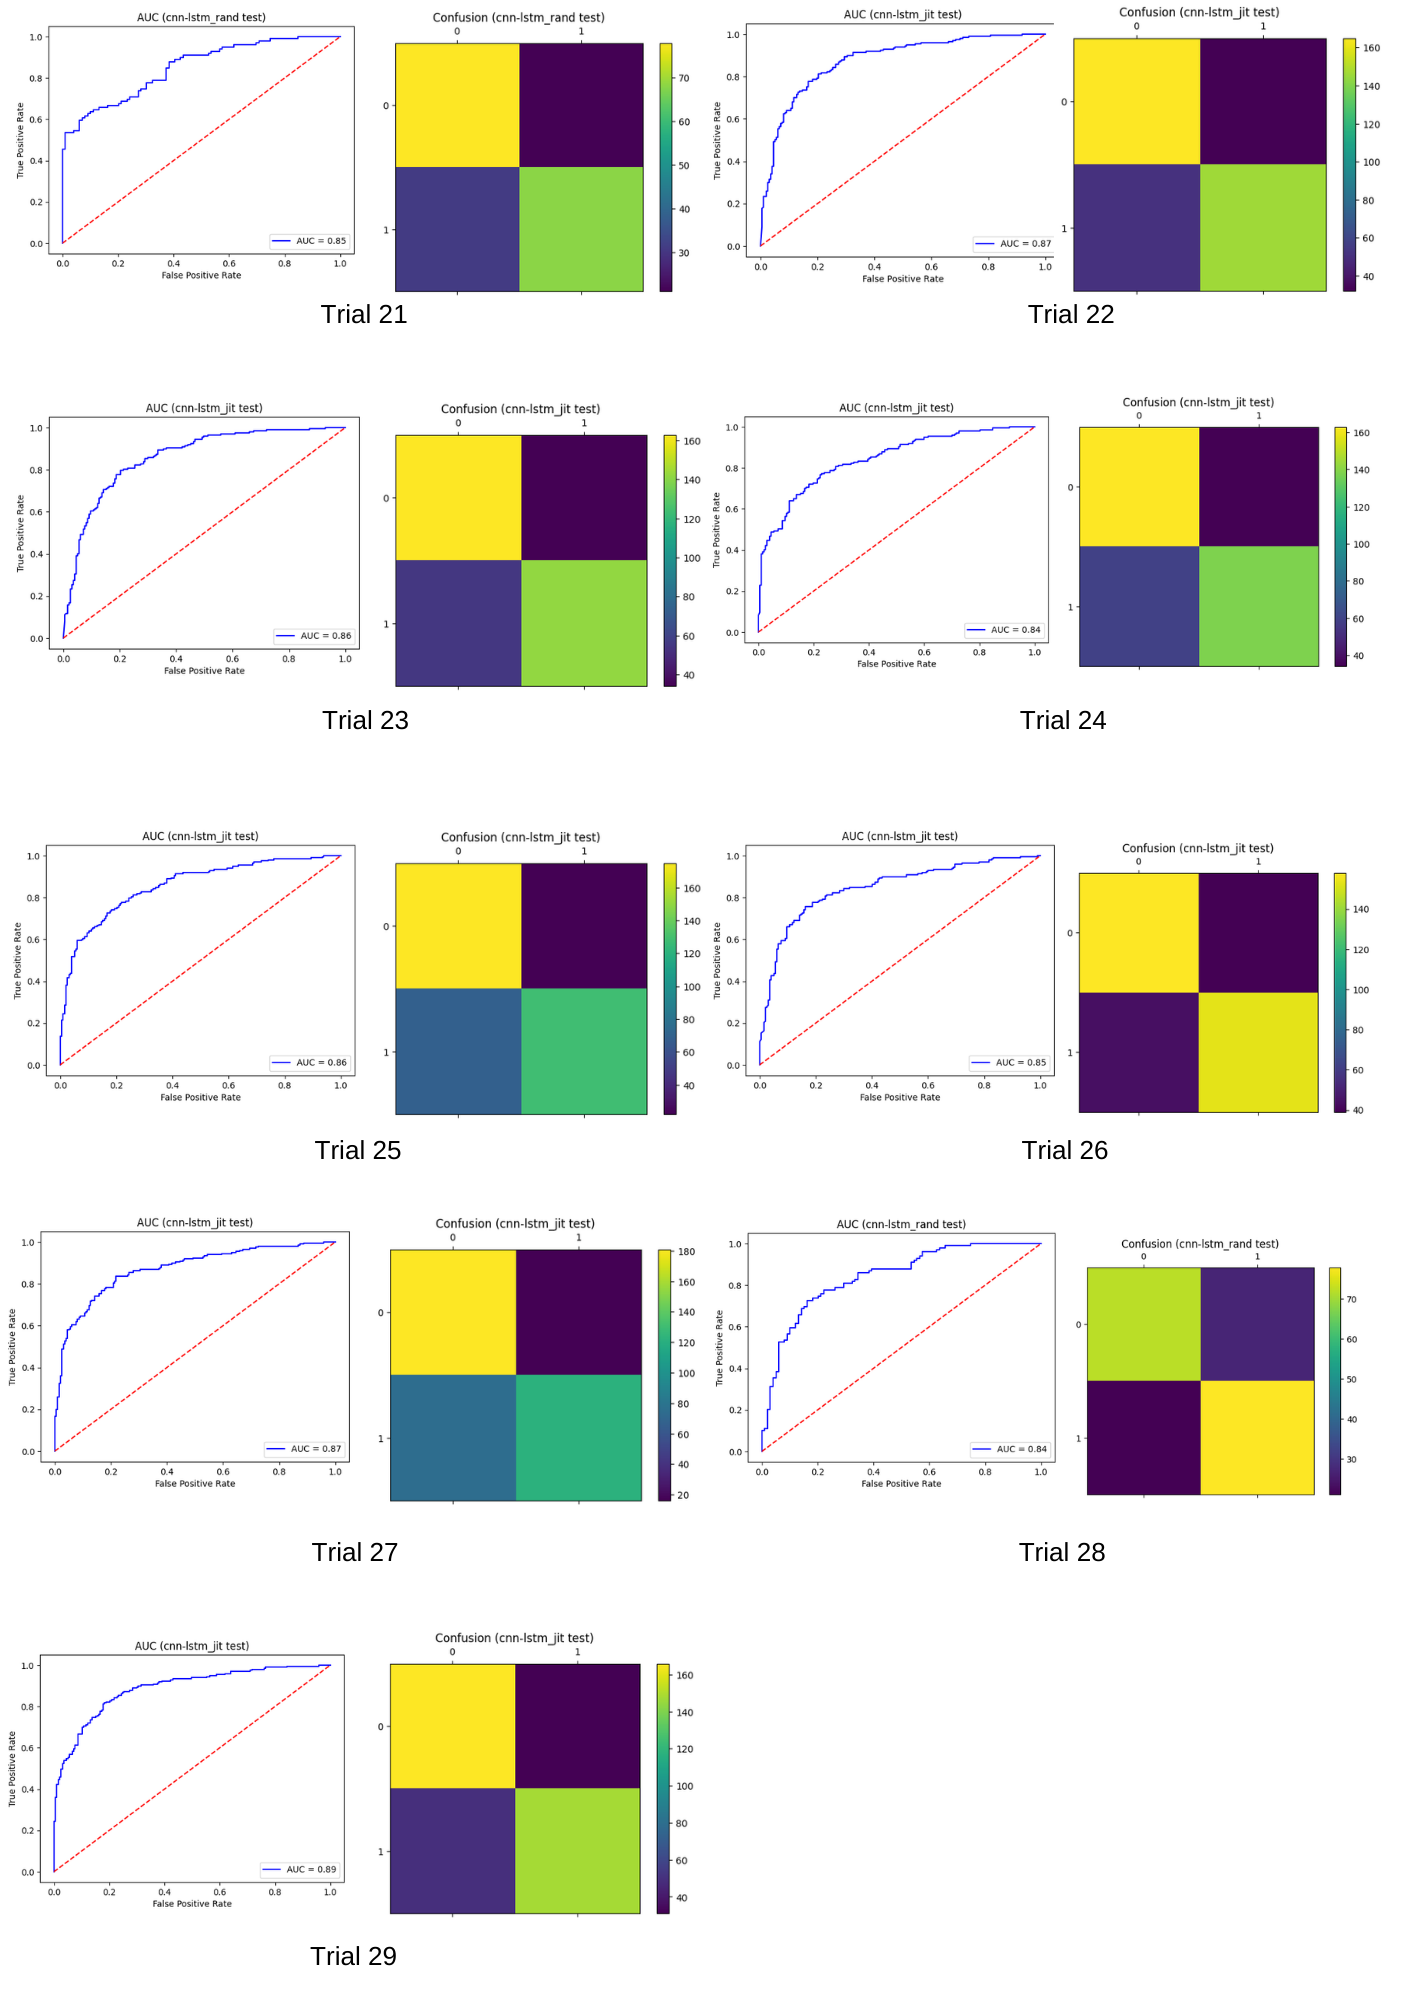
\includegraphics[width=0.9\columnwidth]{figures/cnn-lstm_3.png}
    \label{fig:cnn-lstm_3}
\end{figure}

\end{document}
